\scanpage{42}
2) Cas $n$ impair $\rho=\widetilde\rho$, $\sigma=2\widetilde\sigma$,
l'équation s'écrit
\[
\lambda\widetilde\sigma(2+\lambda\rho)=0.
\]
Donc si $\inserted{\sigma}(=2\widetilde\sigma)$ et $\rho\inserted{(=\widetilde\rho)}$ inv.,
\deleted{la seule} $\exists!$ section $u$ de $U_\rho$, partout $\ne1$,
\deleted{telle} qui invarie $f$, --- ce qui revient au $=$, qui invarie $Q$ --- savoir
\[
\underbrace{u=\operatorname{id}-\frac{2}{\rho}\Pi'\otimes\Pi}_{\text{antipodisme}}
\]
\margin{\uline{NB} Si $\widetilde\sigma$ inv. et non $\sigma$ (\unsure{p. ex.} en car. $2$)
on a \unsure{donc} bien unique solution en $\lambda$, \unsure{savoir que}
$\lambda=-\frac{2}{\rho}$, mais celle-ci peut être nulle en certains pts.
Donner un énoncé commun aux cas $1^\circ)$ et $2^\circ)$ \uline{en termes de}
\figure{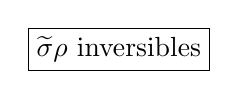
\begin{tikzpicture}
\node[draw,inner sep=3pt] {$\unsure{\widetilde\sigma\rho}$ inversibles};
\end{tikzpicture}}}

D'autre part, conditions \unsure{équivalentes}\deleted{\unsure{alors}}
\deleted{$\unsure{\sigma}$}

a) $2\widetilde\sigma=\sigma=0$ et
$\widetilde\sigma\rho\inserted{(=\unsure{\sigma\widetilde\rho})}=0$

[\uline{NB} Si $2$ inv., ceci équivaut à $\sigma=0$; si $2=0$,
ceci équivaut à $\widetilde\sigma\rho=0$]

b) $U_\rho$ invarie $f^{\mathcal E}$

c) $U_\rho$ \unsure{---} $Q_X$
\margin{\unsure{i.e.}}

Si \deleted{de plus} $\rho=0$, ces conditions équivalent aussi à :

d) $\exists$ \inserted{loc.} section de $U_\rho$ partout $\ne1$ qui
invarie $f^{\mathcal E}$ (ou encore, $Q_X$)
\mspage{41}

